\documentclass[conference]{IEEEtran}

% correct bad hyphenation here
\hyphenation{op-tical net-works semi-conduc-tor}
\usepackage{graphicx} 
\usepackage{subfig}
\usepackage{verbatim}
\usepackage{fancyvrb}
\usepackage{algorithm}
\usepackage{algorithmic}
\usepackage{cite}

\begin{document}

\title{General Expert System Anomaly Detection for Streaming Data}

\author{\IEEEauthorblockN{Andrew Butcher, Oussama Elrawas, Ekrem Kocag\"uneli}
\IEEEauthorblockA{Lane Department of Computer Science and Electrical Engineering\\
West Virginia University, Morgantown, WV 26506\\
abutcher@afrolegs.com, orawas@gmail.com, ekocagun@mix.wvu.edu}}

% make the title area
\maketitle


\begin{abstract}
The effort to model and understand knowledge and data has given rise to a large variety of implementations of knowledge level modeling. 
Aimed at achieving various operations such as anomaly detection, classification and planning, among others, knowledge level modeling allows us to derive generalizations concerning data. 
In this paper, we present a toolkit aimed conducting KL modeling. 
This toolkit will be presented at this stage of its implementation to allow for anomaly detection in classification data.
By using this toolkit, we implemented a two-step, likelihood-based anomaly detector and tested it on simulated classification datasets for various different scenarios.
Our model has achieved to perfectly identify the normal and abnormal test instances from the simulated datasets.
\end{abstract}

\IEEEpeerreviewmaketitle

\section{Introduction}

Expert systems have been proposed to solve various problems in many
different contexts.  Although these systems were developed separately
from each other, all of them share common properties.  The realization
of the properties have led to an exciting idea of \textit{knowledge level modeling} (KL).  
Knowledge level modeling aims to find abstract patterns of inference 
that appear in various expert systems
\cite{Menzies97object-orientedpatterns:}.

In fact the idea of KL is not a very new concept.  In 70s and 80s,
some applications of high level expert systems have been reported.
Although some research was conducted to make this initial work more
common and widely applicable, the current trend of expert system
design usually consists of a somewhat trial and error approach
\cite{Menzies1996}.

Although trial and error method when combined with expert domain
knowledge may yield very successful results, most of these models
require quite a lot of planning, design and research prior to
implementation.  Therefore, the failure to exploit re-usable abstract
domain independent problem solving strategies result in waste of
resources.  Previous research has also adressed this issue and
reported three benefits of using KL modeling
\cite{Menzies97object-orientedpatterns:}:
\begin{itemize}
\item Reuse Benefit:New designs can be bootstratpped from previous designs. 
The new design does not need to be a copy of the previous one and may introduce various new configurations.
However, essential pattern will be reused and be the start point of a new design.
\item Communication Benefit: KL models could be very useful to explain various different expert systems and a novice designer with the knowledge of KL models could easily adapt to a new expert system.
\item Guidance Benefit: By analyzing previous models, designers could get an insight regarding where to direct their focus in the design of a new expert system.
\end{itemize}

The fundamental idea behind KL is that a knowledge base is divided
into two parts: 1) Domain specific facts and 2) domain independent
problem solving strategies \cite{Menzies1996}.  However, a wide range
of current expert system designs are not based on this fundamental
idea and are missing the afore mentioned benefits provided by KL
modeling.

In this research, we are making an analysis of previous KL models and
going further we are proposing a common toolbox that includes common
methods or tools to these models.  After our analysis, we will build
an expert system that will make use of previous KL models and the
necessary methods from the common toolbox of KL models.  The model
will be applied to a world that is perceived by streaming data, which
corresponds to a generalized version of part one for a knowledge base,
i.e. a general representation for domain specific facts.  This will
enable model to be applicable to any specific domain that can be
mapped to the described representative model.

By building this model on the principles of KL modeling, we do not
only exploit the benefits of KL modeling but we also propose a widely
applicable model for a large set of domains.

\section{background}
In this section we will describe and briefly discuss previous work related to the area of knowledge level modelling. As discussed in the introduction, KL modelling is well researched concept and there have been several variations on the theme. KL modelling can be presented in one of two different types of studies and implementations: 

\begin{itemize}
	\item General all encumpassing work on knowledge engineering that attempt to cover and implement a wide range of inference functions. These implementations generally do not target a specific type of data.
	\item Specific work on KL modeling that seek to implement a small subset of functionality. Usually such implementations aim at targeting specific data sets.
\end{itemize}

The more encompassing studies seek to implement extensive KL functionality that is able derive knowledge from most data that is available to their system. such work include the modeling of cognitive processes that is presented in \cite{Clancey1985} by Clancey et. al. In this publication, the authors present flowchart style description to several processes that include:

\begin{itemize}
	\item Diagnosis
	\item Verification
	\item correlation
	\item suitability
	\item classification
	\item Prediction
	\item Repair
	\item Design
	\item Configuration
	\item Planning
	\item Scheduling
\end{itemize}

While implementations to these descriptions are not implemented, it is important to take note of them. Such extensive descriptions represent the tradition of knowledge modeling by way of extensive specification of any knowledge/theory producing process. These processes are briefly explained in following sections. As we will see, our own tool is a is based on his tradition of specification~\cite{riesbeck96}.

Detailing current work regarding this approach to knowledge modeling is currently out of the scope of this paper. However, we will briefly present two papers that lie on either side of the fence of this knowledge modeling equation. 

The first paper \cite{Menzies1996} by Menzies provides a description and a system (HT4) that follows the above tradition and which is done through abduction. Abduction here meaning that rules (or hypotheses) are produced such that, given the final effect/state, we are able to most closely determine our initial effect/state. in other words, we are producing rules that will allow us to produce/ infer old data given our current data. This method is obviously dependent on observing enough data to produce out rules. These rules will ultimately define our knowledge. In a similar manner to the cognitive processes document, this work attempts to apply knowledge modeling to achieve several of the functions mentioned above. Such functions include prediction, classification, explanation, tutoring, planning, monitoring, validation, verification and diagnosis. While not identical to the list of functions mentioned above, it overlaps with regard to most of the functionality. As such, the author presents a general tool for use in KL. Our proposed future implementation will be similar to this, with the main difference being that our method is based on induction.

While this ‎is one side of knowledge modeling, the other side of knowledge modeling forgoes specifying all the above functionality, and instead specifies one rule: remember the past to determine the present \cite{riesbeck96}. This is called Case Based Reasoning (CBR). Argued for by Riesbeck, this method represents knowledge and experience with dealing with that knowledge in the form of case bases that include historical data and actions performed on the data in the past. Current actions are determined by the similarity of our current case/data to previous data. This method is based on the principle that people don't create new decisions based on cognitive analysis, but rather that current actions are based on previous actions conducted in similar situations. 

In the next section we will present a description of the model that we will be using.

%One specific applicatio of knowledge modelling is anomaly detection. Anomaly detection is the process of realizing a change in our current data pattern given knowledge of previous data patterns. This is a very extensive field unto itself, with many different implementations. These implementations can implement anomaly detection using many methods, includign but not restricted to:

%-Classification
%-Clustering
%-Nearest Neighbor
%-Statistics.

%In this section, we will briefly go over a two statistical implementations of anomaly detection. 





\subsection{Library and Toolbox For Design Patterns}
\label{section:library}
KL patterns appear in many different expert systems.  In that respect
the goal of KL modeling can be defined as tpeo identify the abstract
reusable inference skeletons that appear multiple times in such
systems.  A very good example to this concept is the example of
Clancey \cite{Clancey1985}, where he reverse engineered 10 expert
system tools with various different characteristics and found out that
all of them were using the same abstract inference skeleton: Heuristic
classification.  Of course Clancey's example is not the only one.
Another KL methodology KADS \cite{Wielinga1992} was reported to have
been used in more than 40 knowledge-based systems
\cite{Menzies97object-orientedpatterns:}.

Bearing in mind that KL inferece models are used repeatedly in many
different expert systems, it is a good idea to collect and store them.
Clancey proposes a library of pre-defined problem solving strategies
and a a separate knowledge-base that contains domain specific
heuristics \cite{Wielinga1992}.  In this library we can define common
problem solving models that underlie all the expert systems.  When the
common problem solving strategy is combined with separate domain
specific heuristics, then an expert system can easily be built with
less effort.  As examples of models in such a library we can name
verification, incremental configuration, systematic diagnosis and
heuristic classification.

Going further we would also like to mention a toolbox for such a
library that is proposed by Menzies\cite{Menzies2009}.  When we take a
closer look to the library proposed by Clancey \cite{Wielinga1992} we
see that various problem solving models make use of common methods or
algorithms.  For instance verification, classification, sampling
methods, diagnosis, discretization, median and greedy agglomerative
clustering (GAC) are examples to common methods in the toolbox that
can be used by various inference skeletons to form multiple expert
systems in different settings.  We can in fact group these algorithms
in a toolbox that is available to the use of models in the library of
Clancey.

So we can think of building an expert system as a three step process:
\begin{enumerate}
\item Choose a model/template best for your case from the library
\item Pick up required methods from toolbox
\item Insert domain specific heuristics
\end{enumerate}

In our study we will follow the above described three steps to build our model that is capable of processing continuous data and detecting anomalies.
Since we are aiming to provide a generic model, we will not have any domain specific heuristics in our work.
Therefore, we will cover only the first two steps while building our model.

\subsection{Greedy Agglomerative Clustering}
Since the fundamental method in our model will be the greedy
agglomerative clustering (GAC), we will first provide some information
regarding GAC.  Agglomerative, or bottom up, clustering starts with
every individual data point and greedily combines similar points using
a distance metric \cite{Walter}. Our model uses euclidean distance to
pair similar data points. The clusters formed can then be mapped into
a tree structure. A GAC tree partitions the data such that the leaves
in the tree are the original data points and each interior node is a
cluster containing every point in its subtree. The root thus contains
every data point.

When querying the tree we can easily throw away whole subtrees by
comparing our test with the cluster at hand. This speeds up traversal
greatly, allowing for sub-linear query costs.

\section{Our Model}

Our model processes streaming data in chunks of certain number of
instances and tries to find anomalies within the processed data.  For
learning what is abnormal and what is normal, the algorithm relies on
past data and tries to For our case, we use 100 instances in each
chunk, since GAC may have performance drawbacks with datasets that
have more than 100 instances.  While building our model, we will use
the three step procedure that was described in Section
\ref{section:library}.  In the following subsections we will describe
these steps.

\subsection{Select a template from the library}
Since our aim is to find anomalies with this model, we are in fact
dealing with a classification problem where we have two classes:
Normal and abnormal.  The most suitable template for the type of
problem we are tryinig to tackle with is "heuristic classification".

\begin{figure}
\begin{center}
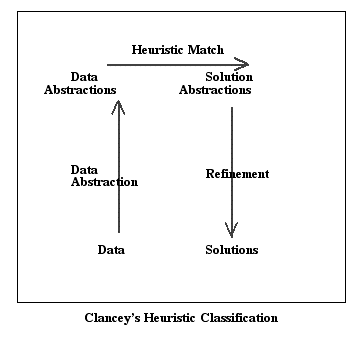
\includegraphics[width=0.5\textwidth]{heuristic_classification.png}
\end{center}
\caption{Heuristic classification takes raw data and applies an
  abstraction. Then on the data abstraction heuristic match methods
  are run, which in our case is a distance based GAC. Then hypothesis
  coming from the heuristic match is evaluated and the solution is
  reached.}\label{fig:heuristic}
\end{figure}

\subsection{Pick up methods from toolbox}
Now we have a basic frame to build our model, but we need to select
the appropriate tools to be able to implement this model.  To abstract
our data we expect the data to be provided to the model in the form of
a two dimensional array in which the rows will correspond to instances
and the columns will correspond to features of the instances.  Then
the data will be normalized to the interval of 0 to 1 and this will
form our abstracted database.  Therefore, we will use a
\textbf{\textit{``normalize''}} method from the toolbox first.

Once the data is normalized, the heuristic match mechanism will start
to work.  Since we are building a GAC tree on the data, we will need a
\textbf{\textit{``GAC''}} method and we will need to calculate the
distances between clusters.  Thus, we will pick up a
\textbf{\textit{``distance''}} function from the toolbox as well.  We
calculate the distance of a single instance to the centroid of
clusters in GAC, and centroids are represented by the mean of all the
features of all the instances in that cluster.  Therefore, we will
also select \textbf{\textit{``mean''}} method of the toolbox.

We now have the template and the required tools to build our expert
system.  The third step would be to insert domain specific heuristics
into the model.  However, the model does not target any domain for the
time being, therefore we will not include this step.

The model whose specifications have been verbally given above is a
generic GAC anomaly detector.  For more detail, we provide the
pseudocode in Figure \ref{figure:trainPseudocode}:

\begin{figure}
\renewcommand{\baselinestretch}{1}
\begin{algorithmic} \footnotesize
\STATE divide dataset into chunks of 100 and process each chunk at a time
\STATE for each chunk run 7 times
\STATE randomize training dataset
\STATE instancei = pick up an instance from in chunki 
\STATE clusters = build a GAC tree from chunki minux instancei instances
\STATE centroidj = mean(clusterj) for all clusters in GAC tree
\STATE calculate the distance of of instancei to all the centroids
\STATE  find closest centroid and see its level in the tree
\STATE if level of closest centroid < floor( \# of all levels in the tree / 2) 
\STATE then give normal class label to instancei
\STATE otherwise give abnormal class label to instancei
\end{algorithmic}
\caption{Pseudocode for training of generic GAC anomaly detector}
\label{figure:trainPseudocode}
\end{figure}

The logic here is that, we want instancei to be closer to majority of
the instances in a tree and not close to leaves, which represent
single/specific cases. If instancei is closer to specific instances
than to a majority, then it is more likely to an anomaly.  We do the
above loop until we process all our dataset. At the end we have
instances at our hand, which make up a normal world according to our
definition.

After the training, we will have 7 labels for each instance in the
chunk of 100 instances. Depending on the majority of the labels,
decide whether an instance is normal or abnormal. Then throw away all
the abnormals. Pick up another chunk and apply the same algorithm We
do the above loop until we process all our dataset. At the end we have
instances at our hand, which make up a normal world according to our
definition.

For testing, use a similar strategy. But this time use the normal
instances that were found before for training. The pseudocode for
testing is given in Figure \ref{figure:testPseudocode}.

\begin{figure}
\renewcommand{\baselinestretch}{1}
\begin{algorithmic} \footnotesize
\STATE randomize our normal world and then make chunks of 100
\STATE build a GAC on chunki
\STATE calculate distance of every test instance to centroids and label them in the same manner to training
\STATE after building a GAC for every chunk and labeling test instances for each chunk, we will have training-size/100 labels for each test instance
\STATE depending on the percentage of labels, we have 3 options for each test instance: 
\STATE decide its normal (if 75\% of the labels indicate its normal)
\STATE decide its abnormal (if 75\% of labels indicate its abnormal) 
\STATE decide that you cannot make a sound decision (if none of the labels exceed 75\%)
\end{algorithmic}
\caption{Pseudocode for testing of generic GAC anomaly detector}
\label{figure:testPseudocode}
\end{figure}

\section{Datasets}

In this research we make use of the following datasets to test our
anomaly dedection model...


\section{Methodology}


\subsection{Anomaly Dedection Train Sets}


\subsection{Anomaly Dedection Anomaly Dedection}



\subsection{Using Train and Test Sets for Anamaly Dedection}



\section{Conclusion}
The conclusion goes here.

% use section* for acknowledgement
\section{Acknowledgment}
We would like to thank...

\bibliographystyle{abbrv}
\bibliography{references}  % sigproc.bib is the name of the Bibliography in this case

\end{document}


